
\section{Short term presynaptic plasticity model}

Assume that the intracellular calcium concentration at the presynaptic terminal follows linear decay dynamics toward a steady state according to
\begin{equation}
        \partial_t c = \frac{c_{\infty}-c}{\tau_c} - k I_{Ca}
        \label{eq:dcdt}
\end{equation}


where $k_c$ ($\mu$M / pC) can be thought of as a rate indicating the impact of the net transmembrane flux of calcium on the intracellular concentration of calcium. As a rule of thumb, the value of $k_c$ should be such that the change in the calcium concentration in a presynaptic terminal after a single action potential could be between 50 and 100  $\mu$M.

Consider synapses in which the probability of activation of the release machinery  depends directly upon binding of calcium, and when unbound, decreases linearly. The dynamics for $r$ can then be
\begin{equation}
   \partial_t r =  \alpha c^n(1-r)-\beta r   \label{eq:dpdt}
\end{equation}

with $\alpha$ in ms$^{-1} \cdot \mu$M$^{-n}$ and $\beta$ in  ms$^{-1}$.
Equation \eqref{eq:dpdt}
can be rewritten as 
\begin{equation}
   \partial_t r = \frac{r_{\infty}(c)-r}{\tau_r(c)} 
\end{equation}
with 
\begin{equation}
    \tau_r(c) = \frac{1}{\alpha c^n + \beta}= \frac{1}{\alpha} \lrRound{\frac{1}{ c^n + \frac{\beta}{\alpha}}} 
\end{equation}
\begin{equation}
r_{\infty}(c) = \frac{c^n}{c^n + \frac{\beta}{\alpha}} 
\label{eq:pInfty}
\end{equation}
The fraction $ \beta/\alpha$ is the calcium concentration at which the steady state for $p$. So let $c_m^n=\beta/\alpha$.
The quantum of released neurotransmiter is proportional to $r$ and the proportion of neurotransmiter ready to be releasable $q$ which is considered as normalized. And whose dynamics is as follow: 

\begin{equation}
\partial_t q =  \frac{q_{\infty}-q}{\tau_q} - r q  \label{eq:dxdt}
\end{equation}

If the recovery of $r$ is fast enough, let $r \approx r_{\infty}(c)$, them the system can be reduced to a 2-d system where dynamic of $r$ is $r_{\infty}(c)$.
The system \eqref{eq:dcdt}-\eqref{eq:dpdt}
\begin{eqnarray}
\partial_t c &=& \frac{c_{\infty}-c}{\tau_c} - k I_{Ca}
\\
\partial_t q &=&  \frac{q_{\infty}-q}{\tau_q} -  r_{\infty}(c) q
\end{eqnarray}
Where $c,r,q$ represent the calcium intracellular concentration, an activation variable of neurotransmitter release and the normalized proportion of neurotransmitter ready to be releasable respectively.
\begin{table}
\begin{tabular}{r r l p{0.75\textwidth}}
Parameter & Value & Units & Description \\
\hline &&&\\
$c_{\infty}$ & 0.050 & $\mu$M & Steady state concentration for intracellular calcium \citep{regehr1995calcium}\\
$q_{\infty}$ & 1.0 & $\mu$M & Steady state for the readily releasable pool\\
$\beta/\alpha$ & \sim 0.001 & ms & \citep{destexhe1994synthesis}
\\
$c_{m}=\lrRound{\beta/\alpha}^{1/n}$ & 50 & $\mu$M & Half activating calcium concentration \\
$ k $ & 0.1  &  & Impact of the voltage-dependent calcium current on the intracellular calcium so that peaks are about 50 $\mu$M \citep{regehr1995calcium} \\
$\tau_c$ & 30.0 & ms & recovery time constant of intracellular calcium concentration\\
$\tau_q$ & 20.0 & ms & Recovery time constant for the readily releasable pool\\
$n$ & 4 & & \citep{}  \\
\hline &&&\\
\end{tabular}
\end{table}


% ------------------------------------
\subsection{Analysis considering delta pulses to predict asymptotic behaviours}
% ------------------------------------
Assume that calcium current behaves like a delta pulse function: 
\begin{equation}
    I_{Ca}= - k_c \sum_{i=1}^n \delta(t-t_i) 
\end{equation}
then system () is: 
\begin{eqnarray} 
\label{eq : deltap}
\partial_t c &=& \frac{c_{\infty}-c}{\tau_c} + k_c \sum_{i=1}^n \delta(t-t_i) \\
\partial_t q &=&  \frac{q_{\infty}-q}{\tau_q} - r_{\infty}(c) q \\
\partial_t r &=& \frac{r_{\infty}(c) - r}{\tau_r}  
\\
r_{\infty}(c) &=& \frac{c^k}{c^k + \frac{\beta}{\alpha}} 
\label{eq : deltapp}
\end{eqnarray}
Calcium dynamics: $c_{\infty} = 0 , c_0 = c(t_0) = k $
\\
Pulse times: $t_0, t_1, ..., t_n$
\begin{eqnarray*}
c_0 &=& c(t_0) = k
\\
c(t) &=& c_0 e^{-(t-t_0)/\tau_c}
=k e^{-(t-t_0)/\tau_c}, \quad t_0\leq t <t_1
\\
c_1 &=& c(t_1) = k \lrRound{1 + e^{-(t_1-t_0)/\tau_c}}
\\
c(t) &=& c_1 e^{-(t-t_1)/\tau_c}, \quad t_1\leq t <t_2
\\
c_2 &=& k+ c_1 e^{-(t_2-t_1)/\tau_c}  
\\
&=& k+ k \lrRound{1 + e^{-(t_1-t_0)/\tau_c}} e^{-(t_2-t_1)/\tau_c} 
\\
&=& k+ k  \lrRound{e^{-(t_2-t_1)/\tau_c}  + e^{-(t_2-t_0)/\tau_c}} 
\\
&=& k \lrRound{1+e^{-(t_2-t_1)/\tau_c}  + e^{-(t_2-t_0)/\tau_c}}
\end{eqnarray*}
Therefore, after the $n$th pulse has arrived,
\begin{eqnarray}
c_n &=& k \lrRound{ 
\sum_{i=0}^{n} e^{-(t_n-t_{i})/\tau_c} 
}
\label{eq:cn}
\\
c(t) &=& c_n e^{-(t-t_n)/\tau_c}, \quad t_n\leq t <t_{n+1}
\label{eq:c(t)tn}
\end{eqnarray}
If pulses are periodic (fixed frequency), with $\delta = t_{i+1}-t_i$, then $t_n - t_0 = n \delta$, and equation~\eqref{eq:cn} transforms into
\begin{eqnarray}
c_n &=& k \lrRound{ 
\sum_{i=0}^{n} e^{-i\delta/\tau_c} 
}
\label{eq:cnPeriodicPulses}
\end{eqnarray}
The quantity $a = e^{-\delta/\tau_c}$ represents the decay factor between pulses for calcium. Then the calcium concentration peak after the $n$th pulse is 
\begin{equation}
c_n=k \lrRound{ 
\sum_{i=0}^{n} a^{i} 
}
= k \lrRound{\frac{1-a^{n+1}}{1-a}}
\label{eq:cAsymptotic}
\end{equation}
For instance, if $\delta=50$ ms and $\tau_c = 10$ ms, then $a=e^{-5}$, which means that there is almost no accumulation of intracellular calcium between pulses at 20 Hz. 

\subsection{Qualitative Analysis of the Autonomous System}

Model \eqref{eq : deltap}-\eqref{eq : deltapp} is a kind of non autonomus differential equation with a finite number of time-dependent moments (delta pulses). Between each delta pulse, the model can be interpreted as a continuous autonomus system which is topologically equivalent to each other defined on different  between pulses  interval. Each of these autonomus systems has the form: 
\begin{eqnarray} 
\partial_t c &=& \frac{c_{\infty}-c}{\tau_c} \\
\partial_t q &=& q \frac{q_{\infty}-q}{\tau_q} - r_{\infty}(c) q 
\end{eqnarray}
whose nullclines are easily calculated:
\begin{eqnarray} 
c &=& c_{\infty}\\
q &=& q_{\infty}-\tau_q r_{\infty}(c) \hspace{1cm} and\\
q &=& 0
\end{eqnarray}
and whose equilibrium points also are easily calculated to be $(0,0)$ and  $(0,x_{\infty})$.
The Jacobian matrix can be expressed as 
\begin{eqnarray}
J[f] &=& \begin{pmatrix}-\frac{1}{\tau_c} & 0 \\
p'(c_a)q & \frac{x_{\infty}-2q}{\tau_q}-r_{\infty}(c_a)
\end{pmatrix}
\end{eqnarray}
so that is possible to known the stability at each point if equilibrium which just depend on the values of parameters  $\tau_c$ and $\tau_q$.
Evaluating the Jacobian matrix at the fixed point $(0,0)$ we obtain 
\begin{eqnarray}
J_{(0,0)}[f] &=& \begin{pmatrix}-\frac{1}{\tau_c} & 0 \\
0 & \frac{q_{\infty}}{\tau_q}
\end{pmatrix}
\end{eqnarray}
so the fixed point is a saddle. While at the point $(0,q_{\infty})$ Jacobian matrix is: 
\begin{eqnarray}
J_{(0,0)}[f] &=& \begin{pmatrix}-\frac{1}{\tau_c} & 0 \\
0 & -\frac{q_{\infty}}{\tau_q}
\end{pmatrix}
\end{eqnarray}
So in this case the fixed point is ever a stable node. As we can see, there is not bifurcations depending on parameters $\tau_q$ or $\tau_c$ at each autonomous model obtained of \eqref{eq : deltap}-\eqref{eq : deltapp}. 
\begin{figure}
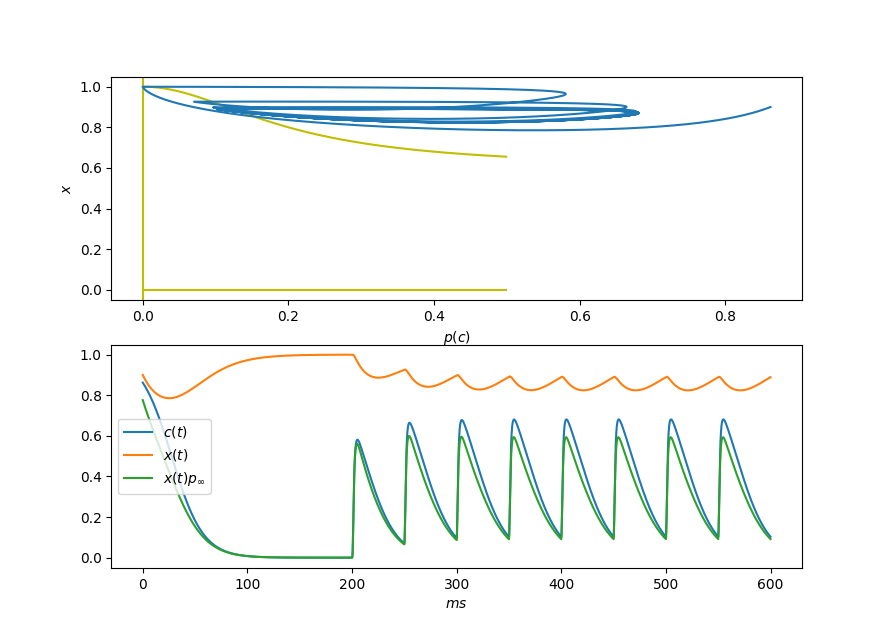
\includegraphics[width=\textwidth]{facilitacion.png}
\caption{phase portrait and temporal courses of a facilitation configuration}
\end{figure}
\begin{figure}
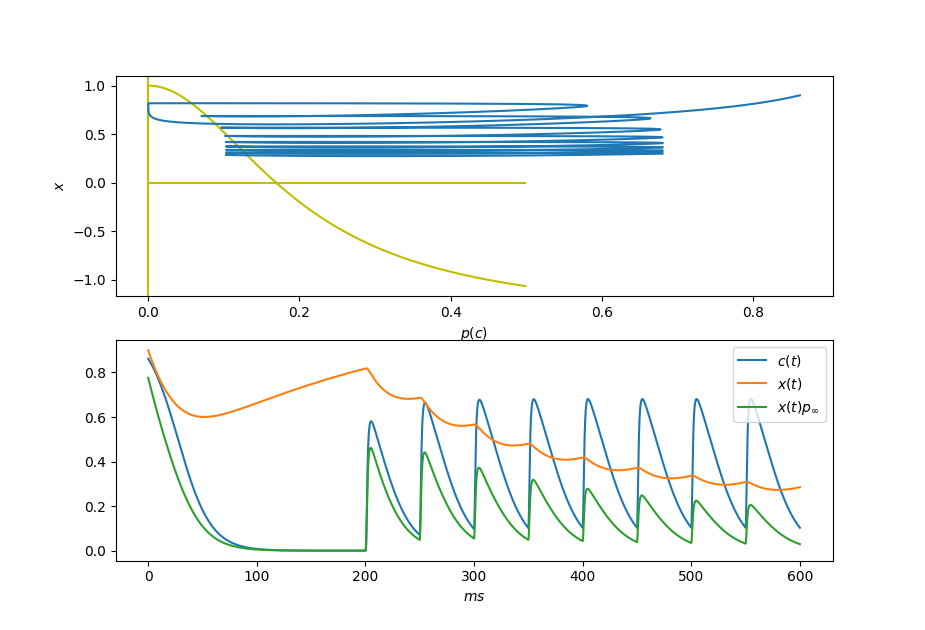
\includegraphics[width=\textwidth]{depression.png}
\caption{phase portrait and temporal courses of a depression configuration}
\end{figure}
